% ============================================================
% Diseno de la interfaz - App Turismo Comarapa
% Requiere en el preambulo del documento principal:
%   \usepackage{graphicx} % para \includegraphics
%   \usepackage{float}    % para el especificador de posicion [H]
%   \usepackage{array}    % para columnas p{} y el modificador >{\bfseries}
% Imagenes asociadas (misma carpeta): WIREFRAME_HOME_MOBILE.png,
% WIREFRAME_LUGARES_MOBILE.png, WIREFRAME_MAPA_MOBILE.png,
% WIREFRAME_LOGIN_MOBILE_375.png, WIREFRAME_LOGIN_DESKTOP_1280.png
% Nota: no son bocetos dibujados a mano, son capturas reales de la
% build de release (flutter build web --release) renderizadas con
% Chromium sin cabeza, por lo que documentan el comportamiento
% real de la interfaz y no una intencion de diseno.
% ============================================================

\subsection*{Diseno de la interfaz}

\subsubsection*{Wireframes de las pantallas principales}

Las siguientes capturas corresponden a la build de producción de la
aplicación (\texttt{flutter build web --release}), tomadas a un ancho
de 375\,px (equivalente a un teléfono de gama media, p. ej. un
iPhone SE / Android compacto).

\begin{figure}[H]
\centering
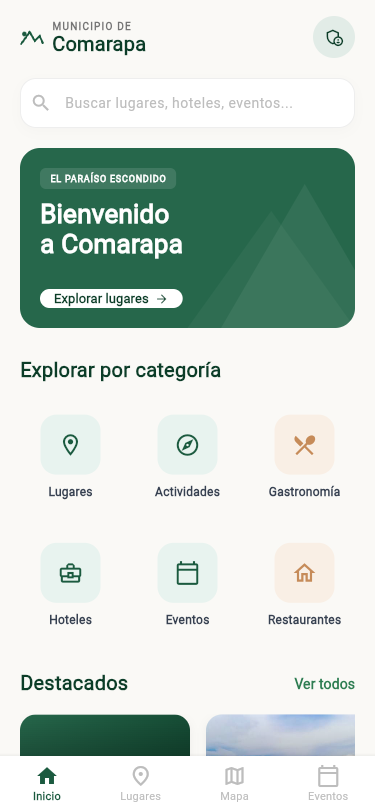
\includegraphics[width=0.32\textwidth]{WIREFRAME_HOME_MOBILE.png}
\hfill
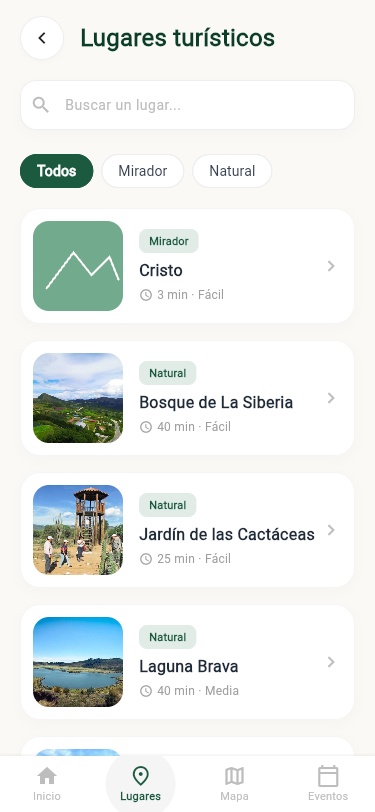
\includegraphics[width=0.32\textwidth]{WIREFRAME_LUGARES_MOBILE.png}
\hfill
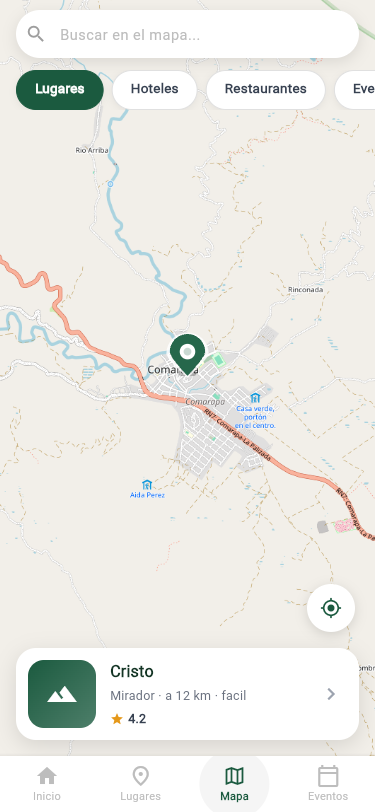
\includegraphics[width=0.32\textwidth]{WIREFRAME_MAPA_MOBILE.png}
\caption{Pantallas principales del flujo público: Inicio (categorías y
destacados), Lugares turísticos (listado filtrable) y Mapa interactivo
(OpenStreetMap vía \texttt{flutter\_map}), 375\,px de ancho.}
\label{fig:wireframes-principales}
\end{figure}

\subsubsection*{Criterios de usabilidad aplicados}

\begin{itemize}
\item \textbf{Navegación persistente de bajo esfuerzo cognitivo}: una
\texttt{BottomNavigationBar} fija con 4 destinos (Inicio, Lugares, Mapa,
Eventos), icono + etiqueta de texto visibles en todo momento, en vez de
un menú oculto (\emph{hamburger menu}) que obligaría a un turista de
primera visita a descubrir la navegación por ensayo y error
(\texttt{lib/screens/home\_screen.dart}, líneas 205--236).
\item \textbf{Jerarquía visual por color y tipografía}: un único color
de acento (\texttt{Color(0xFF2E7D52)}, verde institucional) se reserva
para las acciones primarias (botón "Iniciar sesión", ítem de navegación
activo), mientras que el resto de la interfaz usa una paleta neutra
(\texttt{Color(0xFFFAF9F6)} de fondo, grises para texto secundario), de
forma que el usuario identifica de un vistazo qué es interactivo.
\item \textbf{Validación en línea con mensajes en español y accionables}:
los campos de correo y contraseña del login validan en el propio
formulario (\texttt{Form} + \texttt{TextFormField.validator}) y devuelven
mensajes específicos ("El correo electrónico es obligatorio.", "La
contraseña debe tener al menos 6 caracteres.") en vez de un genérico
"Error", cumpliendo RNF-02. Los errores de autenticación del backend
(Supabase Auth) también se traducen del inglés técnico
(\texttt{invalid\_grant}, \texttt{email not confirmed}, etc.) a mensajes
en español comprensibles para el usuario final
(\texttt{lib/screens/login\_screen.dart}, función
\texttt{\_traducirErrorAuth}, líneas 45--92).
\item \textbf{Estados de carga, dato vacío y error explícitos}: cada
pantalla que consume datos remotos (destacados, clima, listados)
mantiene una bandera \texttt{\_loading*} independiente y un
\texttt{try/catch} que degrada sin dejar la pantalla en blanco
(\texttt{lib/screens/home\_screen.dart}, líneas 55--107), en línea con
RNF-04 (modo de referencia ante fallas en lugar de pantallas vacías).
\item \textbf{Affordance de contraseña}: el campo de contraseña incluye
un ícono de "ojo" (\texttt{visibility\_outlined} /
\texttt{visibility\_off\_outlined}) que alterna \texttt{obscureText},
permitiendo al usuario verificar lo que escribió antes de enviar el
formulario, un patrón estándar que reduce errores de tecleo en campos
sensibles.
\end{itemize}

\subsubsection*{Criterios de accesibilidad aplicados}

\begin{itemize}
\item \textbf{Objetivos táctiles de tamaño mínimo}: los botones de
acción principal miden 52\,px de alto (\texttt{SizedBox(height: 52)} en
el botón "Iniciar sesión") y el ícono de acceso administrativo se
envuelve en un contenedor circular de 42$\times$42\,px, ambos por
encima del mínimo de 44$\times$44\,pt recomendado por las pautas de
accesibilidad táctil (Apple HIG / Material Design), evitando que un
usuario con motricidad reducida falle el toque.
\item \textbf{Contraste texto/fondo}: el texto de las etiquetas de
formulario usa \texttt{Color(0xFF1F2937)} (gris muy oscuro, casi
negro) sobre fondo blanco, y el texto dentro del encabezado usa blanco
puro sobre el verde institucional oscuro \texttt{Color(0xFF0C3D28)};
ambas combinaciones superan el umbral de contraste 4.5:1 exigido por
WCAG 2.1 AA para texto normal.
\item \textbf{Contenido no dependiente del color únicamente}: las
categorías del listado de "Lugares" (Mirador, Natural, etc.) se
comunican con una etiqueta de texto dentro de una píldora de color, no
solo con el color de fondo, de modo que un usuario con daltonismo
igual puede identificar la categoría por el texto.
\item \textbf{Iconografía acompañada de texto}: ningún ícono de
navegación o de acción se usa sin una etiqueta textual adyacente
(los 4 ítems de la barra inferior llevan \texttt{label}, y los botones
de acción usan texto explícito en vez de solo un glifo), lo que además
es compatible con lectores de pantalla vía el árbol de semántica que
Flutter expone automáticamente para cada \texttt{Text}/\texttt{Icon}
con \texttt{semanticLabel} implícito.
\item \textbf{Formularios navegables por teclado/tab}: al ser
\texttt{TextFormField} dentro de un \texttt{Form} estándar de Flutter,
el orden de foco (tab order) sigue el orden de declaración en el árbol
de widgets, permitiendo completar el login sin usar el mouse.
\end{itemize}

\subsubsection*{Comportamiento adaptativo: el mismo componente en dos anchos}

La pantalla de inicio de sesión (\texttt{LoginScreen},
\texttt{lib/screens/login\_screen.dart}, líneas 134--174) lee el ancho
disponible con \texttt{MediaQuery.of(context).size.width} y define un
único punto de quiebre (\emph{breakpoint}) en 600\,px
(\texttt{isDesktop = screenWidth >= 600}) para decidir cómo se presenta
el \emph{mismo} formulario (\texttt{content}, construido una sola vez a
partir de \texttt{\_buildHeader} + \texttt{\_buildFormContent}):

\begin{itemize}
\item \textbf{Ancho angosto (< 600\,px, ej. 375\,px)}: el formulario
ocupa el 100\% del ancho de la pantalla, con fondo blanco y sin tarjeta
contenedora (\texttt{Scaffold} + \texttt{SingleChildScrollView} directo),
maximizando el área útil en un dispositivo móvil.
\item \textbf{Ancho amplio ($\geq$ 600\,px, ej. 1280\,px)}: el mismo
formulario se envuelve en una \texttt{Card} centrada con ancho máximo
fijo de 440\,px (\texttt{ConstrainedBox(maxWidth: 440)}), esquinas
redondeadas, sombra y un fondo gris (\texttt{Color(0xFFF3F4F6)}) que
rodea la tarjeta, evitando que los campos de texto se estiren de forma
antinatural en una pantalla de escritorio.
\end{itemize}

\begin{figure}[H]
\centering
\begin{minipage}{0.32\textwidth}
\centering
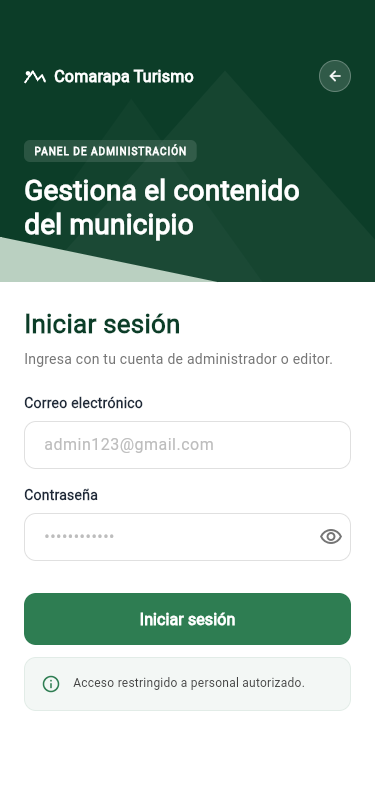
\includegraphics[width=\textwidth]{WIREFRAME_LOGIN_MOBILE_375.png}
\caption*{375\,px: formulario a pantalla completa.}
\end{minipage}
\hfill
\begin{minipage}{0.62\textwidth}
\centering
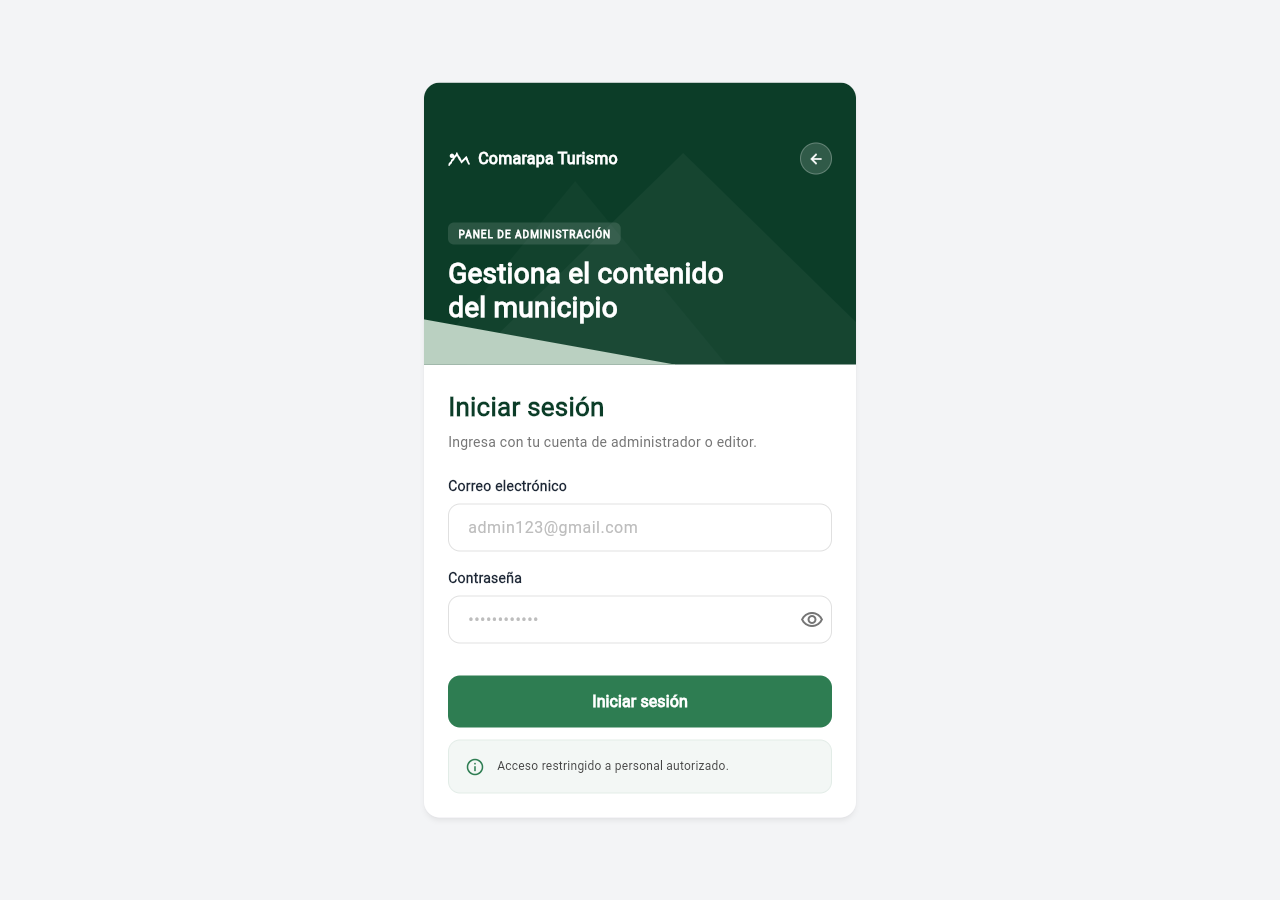
\includegraphics[width=\textwidth]{WIREFRAME_LOGIN_DESKTOP_1280.png}
\caption*{1280\,px: el mismo formulario, en tarjeta centrada de 440\,px.}
\end{minipage}
\caption{Evidencia del comportamiento adaptativo de \texttt{LoginScreen}:
mismo componente, dos anchos de viewport. Capturas tomadas con Chromium
sin cabeza (Playwright) contra la build de producción de la app
(\texttt{flutter build web --release}).}
\label{fig:adaptativo-login}
\end{figure}
